\documentclass[12pt]{article}
\usepackage{amsmath, amsthm, amsfonts, amssymb}
\usepackage{graphicx} % for images
\usepackage{hyperref}
\usepackage{tikz-cd}

% Define theorem and lemma environments
\newtheorem{theorem}{Theorem}
\newtheorem{lemma}{Lemma}
\newtheorem{definition}{Definition}
\newtheorem{corollary}{Corollary}

\setlength{\parindent}{0pt}

\begin{document}

\title{Bayesian-Optimal Multi-Classification implies Abstract Representations (Theory)}

\author{Aman Bhargava}

\date{\today}
\maketitle

\textit{This document outlines the theoretical result from the paper ``Disentangling Representations in RNNs through Multi-task Learning'' by Pantelis Vafidis, Aman Bhargava, Antonio Rangel (coming soon to a preprint server near you!)} \\

% insert figure here -- from media/min_reps_fig_1.png
\begin{figure}[h! tbp]
	\centering 
	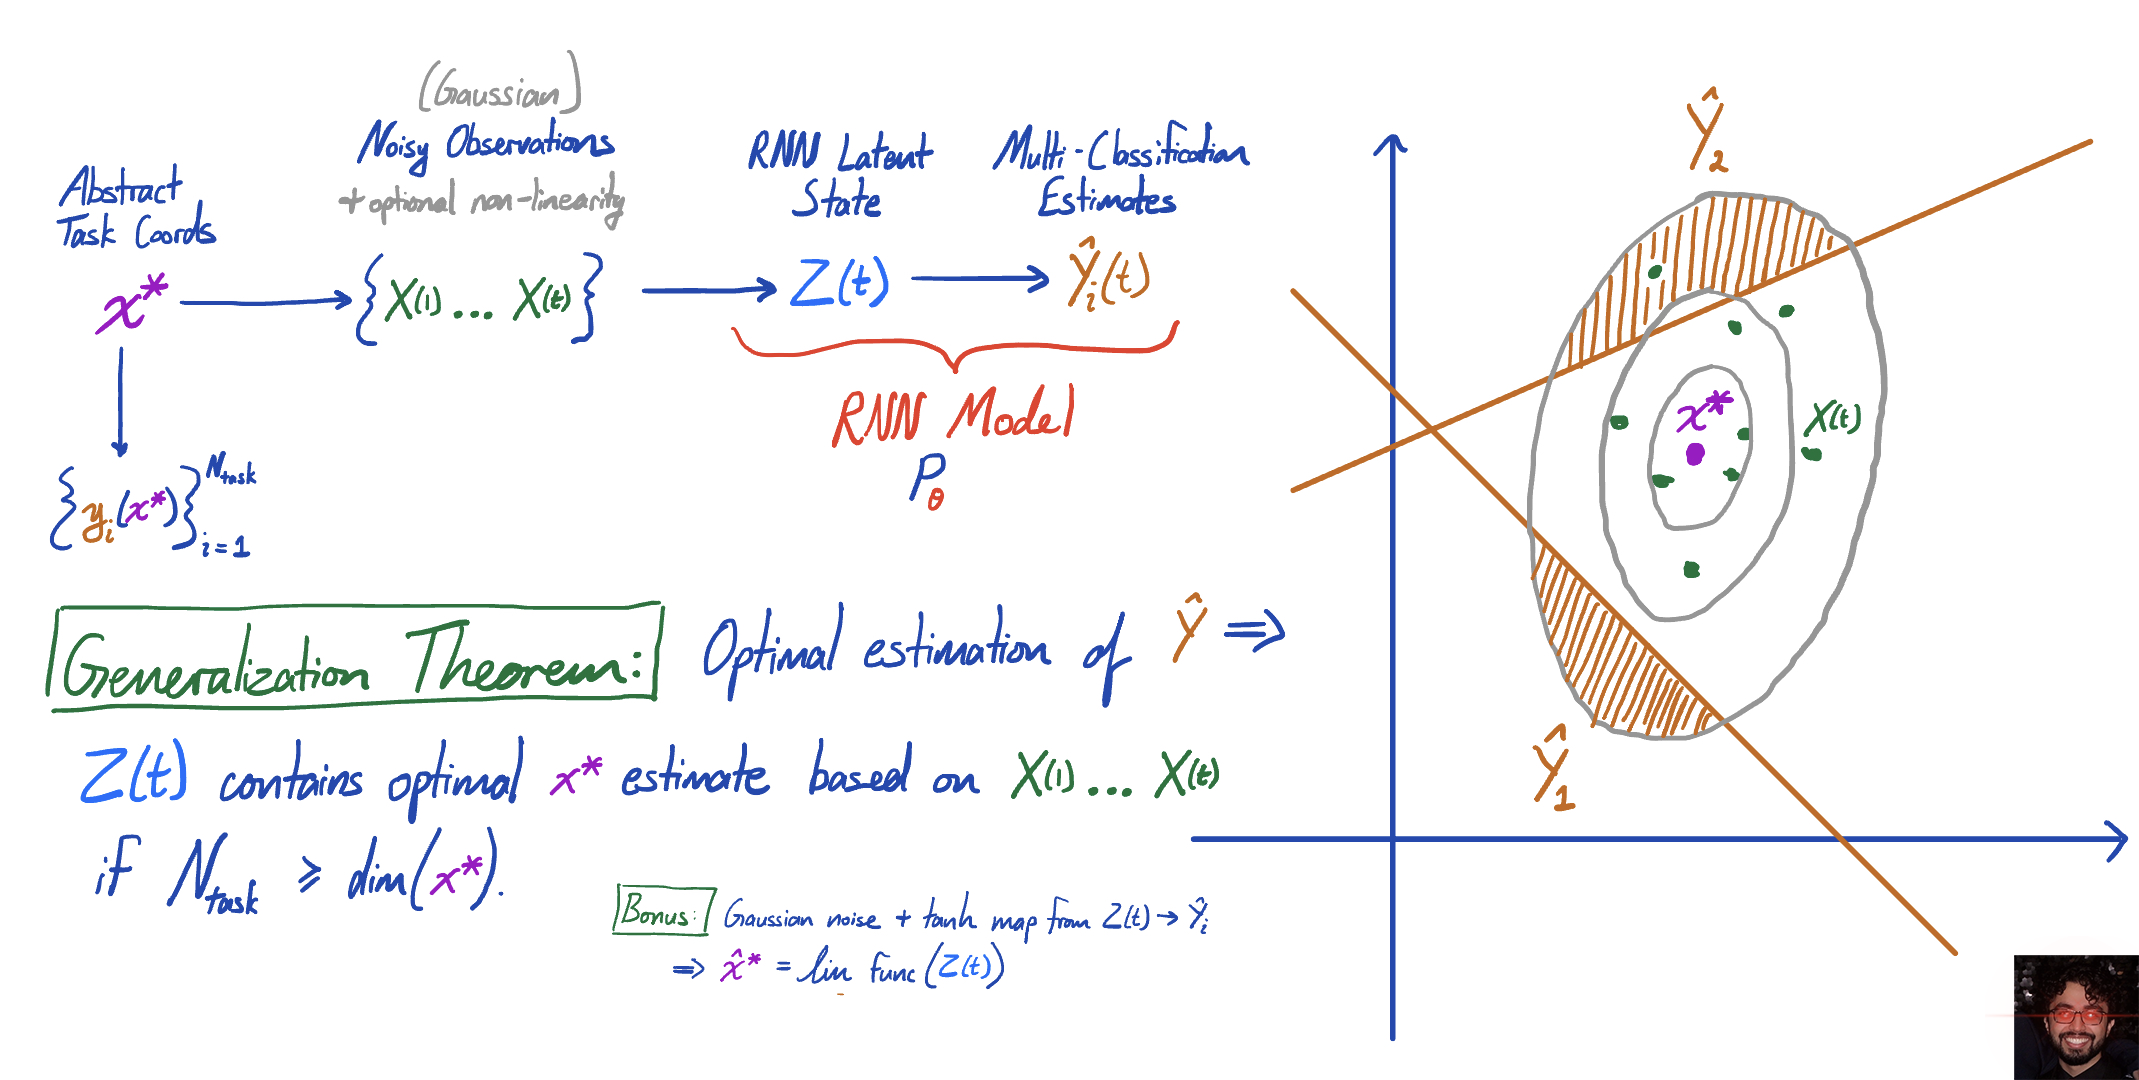
\includegraphics[width=0.9\textwidth]{media/min_reps_fig_1.png}
	\caption{Theoretical framework for optimal multi-task classification. The agent estimates the ground truth decision output $\mathbf y(\mathbf x^*)$ from noisy observations $\mathbf X(t)$, with latent state $\mathbf Z(t)$ encoding an optimal estimate of the de-noised environment state $\mathbf x^*$.}
	\label{fig:1}
\end{figure}

Consider an intelligent agent making decisions in some environment.
The agent receives noisy observations ($\mathbf X(t)$) conditioned on the ``ground truth'' environment state $\mathbf x^*$ (e.g., $\mathbf X(t) \sim f(\mathbf x^* + \eta \mathcal N(0, 1))$ where $f$ is some injective observation map and $\eta$ is the noise level). 
We consider optimal decision making agents that estimate the ground truth decision output $\mathbf y(\mathbf x^*) \in \{0, 1\}^{N_{task}}$ from noisy observations $\mathbf X(t)$). 
Let $\mathbf Z(t)$ represent the latent state of the agent at time $t$ during sequential processing of observations $\mathbf X(t)$. 
We show that \textbf{the agent must represent an optimal estimate of the de-noised environment state coordinate $\mathbf x^*$ in its latent $\mathbf Z(t)$ if the agent optimally estimates decision output $\mathbf y(\mathbf x^*)$ from noisy observations}. 
I thought this was rather surprising, as it generalizes to to any optimal estimator. 
We this result in the case of linear decision boundaries in the multi-classification objective $\mathbf y(\mathbf x^*)$. 
We conclude with a discussion of the implications for non-linear decision boundaries via the introduction of non-linear observation maps $f$ and prove a corollary for agents observing the world through injective (e.g., potentially non-linear and high-dimensional) observation maps $f$.






\section{General, Non-Linear Problem Statement}
\label{sec:intro}


\paragraph{Noisy Multi-Classifier: } Formalize the ``environment state'' as $X
\sim P(X)$ with sample space $\mathcal X$ and a corresponding ground truth 
decision set $P(Y_i | X)$ for $i\in [N]$ (e.g., multi-classification on
the environment state). 
Denote the i.i.d. noise process $X_i \sim P(\tilde X_i | X)$ from which
observations $\tilde X_i$ are sampled. 
We consider optimal estimators of the ground truth readout $Y$ given noisy
measurements $\tilde X$ denoted $P(\hat Y | \tilde X_1, \dots, \tilde X_T)$. 


\begin{equation}
	\label{eqn:prob_statement}
	% X \to \tilde X \to \hat Y
	\begin{tikzcd}
		X \arrow[rd] \arrow[r, "\text{noise}"] & \{\tilde X_t\}_{t\in [T]} \arrow[r, "\text{agent}"] & \{\hat Y_i\}_{i\in [N]}\\
		& \{Y_i\}_{i\in [N]}
	\end{tikzcd}
\end{equation}


\paragraph{Geometry: } Let $X$ reside in a metric space $\mathcal X$. 
Let each $Y_i$ be defined in terms of a binary discriminator $\phi_i: \mathcal X \to \{0, 1\}$. 
Let the equivalence classes of $\mathcal X$ under each discriminator $\phi_i$ be connected (i.e., $\{x | \phi_i(x) = 1, x\in \mathcal X\}$ is connected for each $\phi_i$).


\paragraph{Linearity: } We will begin by presenting a proof on the case where
the decision boundaries are linear. Note that this may be readily generalized
to non-linear decision boundaries by considering the linear approximation of
the decision boundaries in the vicinity of the true environment state, or by
inserting an injective non-linear map from some abstract coordinate space
$\mathcal X^*$ to observation space $\mathcal X$. 


\begin{figure}[h! tbp]
	\centering 
	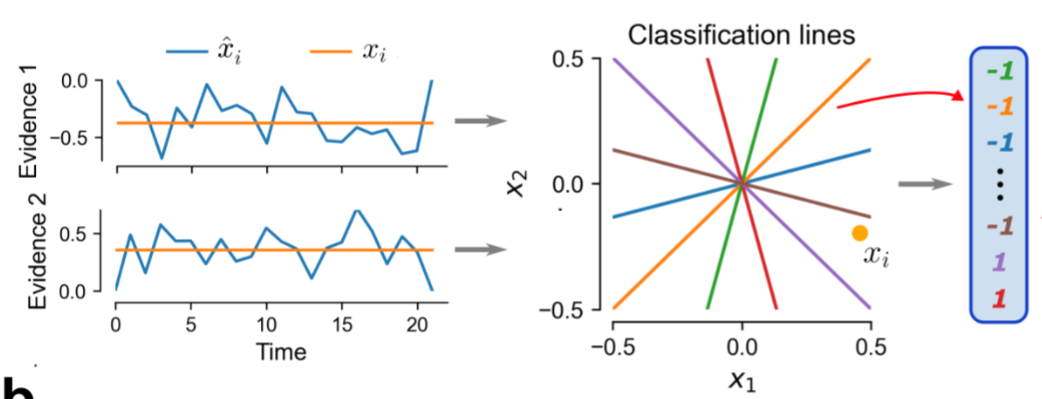
\includegraphics[width=0.9\textwidth]{media/multitask_fig2a.png}
	\caption[Multitasking RNN learns abstract representations]{\textbf{Multitasking RNN learns abstract representations. } Data generating process. The task is to simultaneously report whether the true joint evidence $(x_1,x_2)$ (yellow dot) lies above ($+1$) or below ($-1$) a number of classification lines (here 6).}
	\label{fig:2a}
\end{figure}


% 
We seek to understand the properties of optimal multi-classifiers in the paradigm illustrated in Figure~\ref{fig:2a} where an estimate of classification certainty is made. 
We denote the set of classification estimates as $\hat{\mathbf Y}$, a vector of Bernoulli random variables. 
We prove that \textbf{any optimal multi-task classifier} with i.i.d. noisy inputs $\mathbf X(1), \dots, \mathbf X(t)$ \textbf{implicitly estimates the ground truth coordinate $\mathbf x^*$ in its latent state $\mathbf Z(t)$}. 

\begin{equation}
    \mathbf x^* 
    \to \{\mathbf X(t)\} 
    \to \mathbf Z(t)
    \to \hat{\mathbf Y}(t)
\end{equation}

Specifically, we prove that $\mathbf Z(t)$ represents the optimal estimate of $\mathbf x^*$ given the noisy measurements as long as the classification boundary normal vectors span the input space. 
For random decision boundaries in $D$-dimensional input space, we would expect $D$ classification boundaries to satisfy this condition.\\


This result holds for \textit{any} system that performs optimal multi-task classification with a latent variable separating the inputs from the outputs (e.g., RNNs, Bayesian filters, etc.), \textbf{regardless of the internal dynamics of the latent state}.



\section{Trilateration Theorem for Linear Decision Boundaries}

\textit{Presented in Appendix B of ``Disentangling Representations in RNNs through Multi-task Learning''} \\


\textit{\textbf{Notation:} lower case variables denote scalars (e.g., $x$), upper case variables denote random variables (e.g., $X$), and boldfaced variables denote vector quantities (e.g., $\mathbf x, \mathbf X$). 
We denote the $D\times D$ identity matrix as $\mathbf I_d$.} \\

\paragraph{Variable Glossary: }
\begin{itemize}
    \item $\mathbf x^* \in \mathbb R^D: $ Ground truth (un-noised) input variable.
    \item $\mathbf X(t) \sim \mathbf x^* + \sigma \mathcal N(\mathbf 0, \mathbf I_d)$ are i.i.d. noisy measurements of $\mathbf x^*$, where 
    \begin{itemize}
        \item $\sigma$ is the amount of equivariant Gaussian noise, and 
        \item $t$ is the discrete time index within a trial.
    \end{itemize}
    \item $N_{task}$ is the number of classification tasks, 
    \item $\{(\mathbf c_i, b_i)\}_{i=1}^{N_{task}}$ are the classification boundary normal vectors and offsets respectively, with $\mathbf c_i \in \mathbb R^D$ and $b_i\in \mathbb R$. We assume each $\| \mathbf c_i \| = 1$.
    \item $(\mathbf C, \mathbf b)$ are a matrix and vector representing each of the $N_{task}$ classification tasks where $\mathbf C\in \mathbb R^{N\times D}$ 
    \item  $\mathbf y(\mathbf x^*) \in \{-1, +1\}^{N_{task}}:$ Ground truth classification outputs, where each ground truth classification $y_i(\mathbf x^*)$ is given by 
        \begin{equation}
        	\label{def:decision_rule}
        	y_i(\mathbf x) = \begin{cases}
        		+1 & \text{ if } \mathbf c_i^\top \mathbf x > b_i \\ 
        		-1 & \text{ otherwise } 
        	\end{cases}
        \end{equation}

    \item $\mathbf Z(t): $ Latent variable of a multi-task classification model, conditional on $\mathbf X(1), \dots, \mathbf X(t)$. 
    \item $\hat{\mathbf Y}(t) \in [0, 1]^{N_{task}}: $ Output vector of the multi-task classification model at time $t$, where each $\hat Y_i(t)$ is a Bernoulli random variable parameter representing the conditional probability $\Pr\{y_i(\mathbf x^*) = +1\}$ given the noisy observations (via latent variable $\mathbf Z(t)$ -- see graphical model in Equation~\ref{eqn:full_picture}). 
    \item $\hat{\mathbf X}(t) = \mathcal N(\mu(t), \Sigma(t)): $ Optimal estimate of $\mathbf x^*$ given measurements $\mathbf X(1), \dots, \mathbf X(t)$, derived in Lemma~\ref{lemma:x_star_estimate}. 
    % \begin{itemize}
    %     \item $\mu = \text{mean}(\mathbf X(1), \dots, \mathbf X(t))$ 
    %     \item $\Sigma = t^{-1} \sigma \mathbf I_d$
    % \end{itemize}
\end{itemize}

\paragraph{Problem Statement: } We consider optimal estimators of $\mathbf y(\mathbf x^*)$ in the multi-classification paradigm in Equation~\ref{eqn:full_picture}, shown graphically in Figure~\ref{fig:2a}. 
\begin{equation}
    \label{eqn:full_picture}
    \mathbf x^* 
    \to \{\mathbf X(1), \dots, \mathbf X(t)\} 
    \to \mathbf Z(t) 
    \to \hat{\mathbf Y}(t)
\end{equation}





\begin{figure}[h! tbp]
	\centering 
	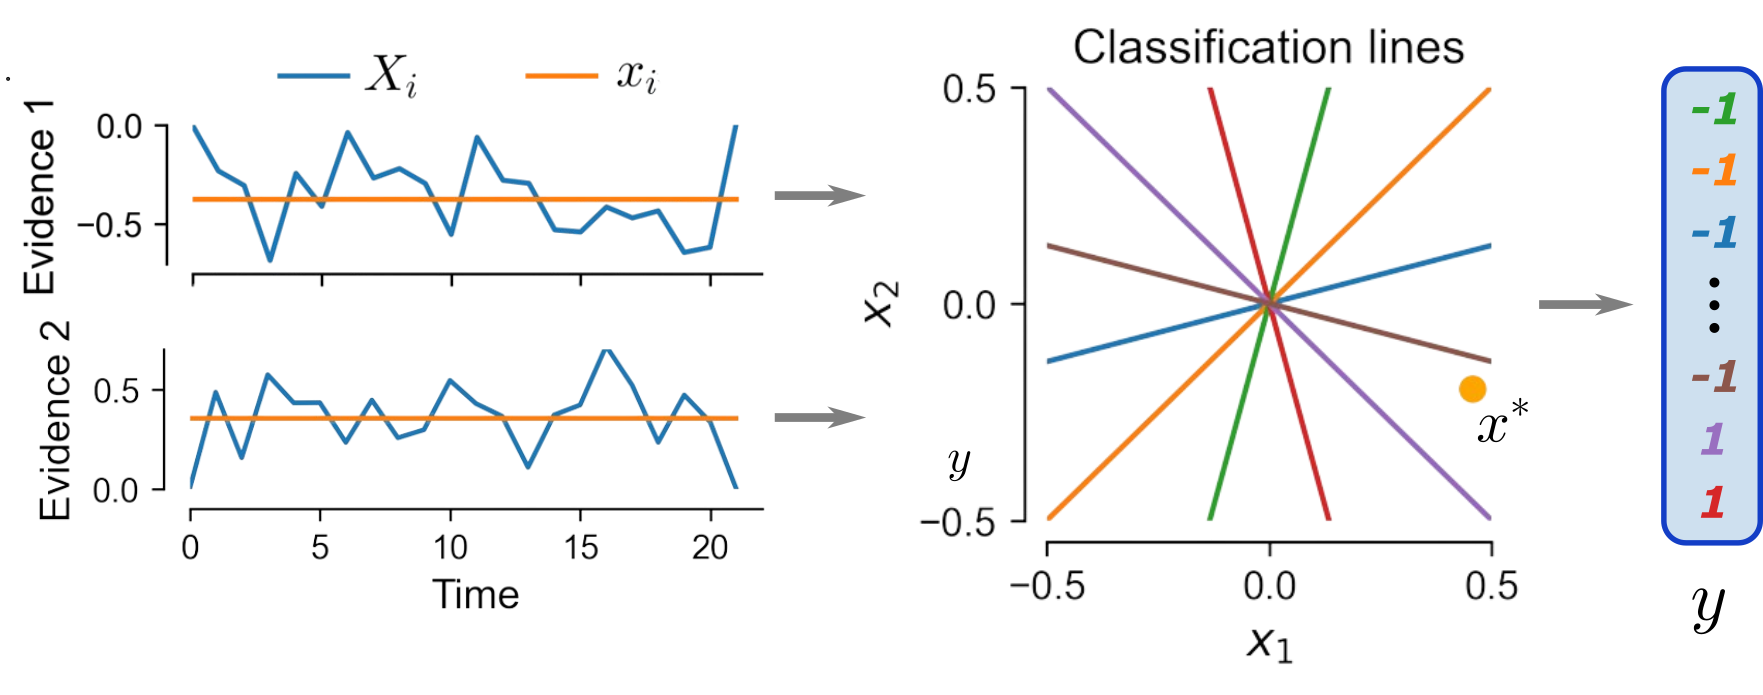
\includegraphics[width=0.7\textwidth]{media/data_gen.png}
	\caption{Data generating process. The task is to simultaneously report whether the true joint evidence $\mathbf x^* = [x_1,x_2]^T$ (yellow dot) lies above ($+1$) or below ($-1$) a number of classification lines (here 6).}
	\label{fig:2a}
\end{figure}


\paragraph{Contribution: } We derive optimal classification estimates $\hat{\mathbf Y}(t)$ in Lemma~\ref{lemma:zscore}. We show that the mean $\mu$ of $\hat{\mathbf X}(t)$ -- the optimal estimator of $\mathbf x^*$ -- can be reconstructed from $\hat{\mathbf Y}(t)$ in Theorem~\ref{thm:main}. Finally, we show via the data processing inequality that latent variable $\mathbf Z(t)$ must contain all information about $\mu$ for any system that produces optimal $\hat{\mathbf Y}(t)$. 








\subsection{Single Decision Boundary}
\label{sec:single_boundary}

First, we will derive $\hat Y(t)$ for a single decision boundary with parameters $(\mathbf c, b)$. 
We focus on $P(\hat Y(t) | \mathbf X(1), \dots, \mathbf X(t))$, reintroducing the latent variable $\mathbf Z(t)$ later on. 

Since $y(\mathbf x^*)$ is a deterministic function of non-random variable $\mathbf x^*$, we will derive the probability distribution over $P(\mathbf x^* | \mathbf X(1), \dots, \mathbf X(t))$ -- denoted $\hat{\mathbf X}(t)$ -- to determine $\hat Y = y(\hat{\mathbf X}(t))$
\footnote{Note that the intermediate computation of $\hat{\mathbf X}(t)$ does not imply that a system \textit{must} compute this value to predict $\hat Y$, as the full computation of $\hat{\mathbf X}(t)$ may not be necessary to determine $\hat Y(t)$.}.


\begin{lemma}
    \label{lemma:x_star_estimate}
	Assuming no prior on $\mathbf x^*$, the conditional probability distribution $\hat{\mathbf X}(t) \sim P(\mathbf x^* | \mathbf X(1), \dots, \mathbf X(t))$ is given by 
	\begin{equation}
		\hat{\mathbf X}(t) = \mathcal N(\mu(t), \Sigma(t))
        \label{eqn:estimator}
	\end{equation}

	where $\mu(t)= \text{mean}(\mathbf X(1), \dots, \mathbf X(t))$ and $\Sigma(t) = t^{-1} \sigma^2 \mathbf I_d$. 

	\begin{proof}
		Since $\mathbf X(1), \dots, \mathbf X(t)$ are i.i.d. from a Gaussian distribution with mean $\mathbf x^*$ and identity covariance, the sample mean is known to be distributed normally centered at the ground truth $\mathbf x^*$. 
		We apply the known standard deviation of the underlying distribution (identity covariance scaled by $\sigma$) to arrive at $\Sigma(t) = t^{-1} \sigma^2 \mathbf I_d$ as the variance on the sample mean (derived from the central limit theorem). 
	\end{proof}
\end{lemma}


We can use estimator $\hat{\mathbf X}(t)$ to construct $\hat{\mathbf Y}(t)$ by expanding $\hat{\mathbf Y}(t) = y(\hat{\mathbf X}(t))$ via Equation~\ref{def:decision_rule}. 

In essence, we are interested in the amount of the probability density of $\hat{\mathbf X}$ that lies on each side of the decision boundary. 
Deriving this probability is simplified by the fact that $\hat{\mathbf X}$ is isotropic -- i.e., it inherits the spherical covariance of the underlying data generation process (Lemma~\ref{lemma:zscore}). 



\begin{lemma}
	\label{lemma:zscore}
	$\hat{\mathbf X}(t) = \mathcal N(\mu(t), \Sigma(t))$ with isotropic covariance $\Sigma(t) = t^{-1} \sigma^2 \mathbf I_d$ and mean $\mathbf \mu(t) \in \mathbb R^D$.
	The probability density of $\hat{\mathbf X}(t)$ on the positive side of the decision boundary $\{\mathbf x : \mathbf c^\top \mathbf x > b\}$ can be expressed as 
	\begin{equation}
		\label{eqn:class_prob}
        \hat Y(t) \triangleq
		\Pr\{\mathbf c^\top \mathbf x^* > b\} = \Phi(k\sqrt{t} / \sigma)
	\end{equation}
	where $\Phi$ is the CDF of the normal distribution and $k = \mathbf{c^\top}\mu(t) - b$ is the signed projection distance between the decision boundary and the mean $\mu(t)$ of $\hat{\mathbf X}(t)$. 
\end{lemma}
\begin{proof}
	Since the $\hat{\mathbf X}(t)$ is isotropic, the variance on every axis is equal and independent. 
	We may rotate our coordinate system such that the projection line between the plane and the mean of $\hat{\mathbf X}(t)$ aligns with an axis we denote as ``axis 0''. 
	The rest of the axes must be orthogonal to the plane. 
	Since each component of an isotropic Gaussian is independent, the marginal distribution of $\hat{\mathbf X}(t)$ on axis 0 is a univariate Gaussian with variance $t^{-1} \sigma^2$ mean at distance $k$ from the boundary. 
	Equation~\ref{eqn:class_prob} applies the normal distribution CDF $\Phi$ to determine the probability mass on the positive side of the boundary. 
\end{proof}


% Thus we are able to construct our optimal estimator $\hat{Y}(t)$ for $P(y(\mathbf x^*) | X(1), \dots, X(t))$ using lemma 1 as 
% \begin{equation}
% 	\label{eqn:single_estimator}
% 	\hat{Y} = \begin{cases}
% 		+1 & \text{ with probability } \Phi\big( 
% 			k \sqrt t / \sigma
% 			\big)\\ 
% 		-1 & \text{ otherwise } 
% 	\end{cases}
% \end{equation}


Observe that $\hat Y(t)$ in Equation~\ref{eqn:class_prob} \textbf{monotonically scales} with the signed distance $k$ between the hyperplane and $\mathbf \mu(t)$ (CDFs are monotonic). 

\begin{lemma}
	\label{lemma:prob_to_dist}
	Knowledge of time $t$ and optimal classification estimate $\hat Y(t)$ is sufficient to determine the projection distance $k$ between $\mathbf \mu(t) = \text{mean}\big(\mathbf X(1), \dots, \mathbf X(t)\big)$ and the decision boundary $(\mathbf c, b)$. 
\end{lemma}
\begin{proof}
	Recall Equation~\ref{eqn:class_prob} from Lemma~\ref{lemma:zscore}. 
	We may solve for projection distance $k$ separating the decision boundary and the mean $\mathbf \mu(t)$ of observations $\mathbf X(1), \dots, \mathbf X(t)$ as 
	\begin{equation}
		\label{eqn:solve_proj_dist}
		k = \frac{\sigma}{\sqrt t}\Phi^{-1}(\hat Y(t))
	\end{equation}

	Since $\Phi$ is the CDF of the normal distribution, and the normal distribution is not zero except at $\pm \infty$, the inverse $\Phi^{-1}$ is well-defined.
\end{proof}


\subsection{Trilateration via Multiple Decision Boundaries}

\paragraph{To recap Section~\ref{sec:single_boundary}}: We derived an optimal estimator of $\mathbf x^*$ (denoted $\hat{\mathbf X}(t)$) based on noisy i.i.d. measurements $\mathbf X(1), \dots, \mathbf X(t) \sim \mathcal N(\mathbf x^*, \sigma^2 \mathbf I_d)$ in Lemma~\ref{lemma:x_star_estimate}. 
In Lemma~\ref{lemma:zscore} we derived the equation for Bernoulli variable $\hat{Y}(t)$ to estimate a single classification output $y(\mathbf x^*)$ based on the same noisy measurements via $\hat{\mathbf X}(t)$.
Finally, we showed in Lemma~\ref{lemma:prob_to_dist} that the uncertainty in $\hat{Y}(t)$ and the time $t$ is sufficient to determine the projection distance between the decision boundary and $\mu(t) = \text{mean}(\mathbf X(1), \dots, \mathbf X(t))$ via Equation~\ref{eqn:solve_proj_dist}. \\


Let $\hat{\mathbf Y}(t)$ denote the vector of classification estimates $\hat Y(t)$ from Equation~\ref{eqn:solve_proj_dist}. We now have the tools to prove our final result via \textbf{trilateration}. Much like distance information from cell towers can be used to trilaterate\footnote{Trilateration differs from triangulation, and it is more frequently used in practice. Triangulation is when one has angle information w.r.t. the cell towers. Usually, this is not available -- so one \textbf{trilaterates} their position \cite{oguejiofor2013trilateration}. This more closely matches our setting, where we just have distances information w.r.t. the decision boundaries and must determine the position.} one's position, we will leverage Lemma~\ref{lemma:prob_to_dist} and use distances from decision boundaries $\{(\mathbf c_i, b_i)\}_{i\in [N_{task}]}$ to constrain the positions.

\begin{theorem}[Trilateration Theorem]
	\label{thm:main}
	% Consider the problem statement from above with optimal multi-task classification output $\hat{\mathbf Y}(t)$. 
    % Let $\mathbf C$ be the matrix of decision boundaries with row vectors $\mathbf c_i$ (cf Equation~\ref{def:decision_rule}). 
	If $\mathbf C$ is full-rank, then $\hat{\mathbf Y}(t)$, $t$, $\mathbf b$, and $\mathbf C$ are sufficient to reconstruct the exact value of $\mathbf \mu(t)$, the mean of $\mathbf X(1), \dots, \mathbf X(t)$, which is also the optimal estimator for $\mathbf x^*$. 
\end{theorem}
\begin{proof}
	We may prove this claim by providing an algorithm to reconstruct $\mathbf \mu(t) = \text{mean}(\mathbf X(1), \dots, \mathbf X(t))$ from $\hat{\mathbf Y}(t), \mathbf C$, and $t$.
	Invoke Lemma~\ref{lemma:prob_to_dist} to compute the signed projection distance between $\mathbf \mu(t)$ and each decision plane $(\mathbf c_i, b_i)$.
	Let $\mathbf k = [k_1, \dots, k_M]^\top$ where each $k_i$ corresponds to decision boundary $\mathbf c_i$.
    Then the mean $\mathbf \mu(t)$ must satisfy 
	\begin{equation}
		\label{eqn:final_lin_sys}
		\mathbf {C \mu(t)} = \mathbf k + \mathbf b 
	\end{equation}
	Thus, for full rank $\mathbf C$, we will have a uniquely determined $\mu(t)$ value. 
\end{proof}


\begin{theorem}[General Representation Theorem]
\label{thm:data_proc_ineq}
    Any system that optimally estimates $\hat{\mathbf Y}$ based on noisy measurements $\{\mathbf X(1), \dots, \mathbf X(t)\}$ must implicitly encode a representation of optimal estimator $\mu(t) = \text{mean}(\mathbf X(1), \dots, \mathbf X(t))$ in its latent state $\mathbf Z(t)$ if decision boundary matrix $\mathbf C$ is full rank. 
	% For any system implementing optimal Bayesian filtering to estimate $\hat{\mathbf{Y}}(t)$ based on latent $\mathbf Z(t)$ and inputs $\{\mathbf X(0), \dots, \mathbf X(t)\}$, the latent variable $\mathbf Z(t)$ must necessarily encode a representation of the mean $\mu$ of optimal $\mathbf x^*$ estimator $\hat{\mathbf X}$, where $\hat{\mathbf X} \sim \mathcal{N}(\mu, \Sigma)$, and
	% \begin{align*}
	% 	\mu &= \text{mean}\left(\mathbf X(1), \dots, \mathbf X(t)\right), \\
	% 	\Sigma &= \hat{\Sigma} = t^{-\frac{1}{2}} \mathbf{I}_d.
	% \end{align*}
\end{theorem}

\begin{proof}
	This follows from the data processing inequality. We  begin with the following Markov chain: 
	\begin{equation}
		\mathbf x^* \to \{\mathbf X(1), \dots, \mathbf X(t)\} \to \mathbf{Z}(t) \to \hat{\mathbf{Y}}(t) \to \mu(t) 
	\end{equation}
    Put more simply, we have $\mathbf x^* \to \mathbf Z(t) \to \mu(t)$. 
    Applying the data processing inequality, we obtain 
    \begin{equation}
        \label{eqn:data_proc_ineq}
        I\big( \mathbf x^*; \mathbf Z(t) \big) \geq I\big( \mathbf x^*;  \mu (t) \big)
    \end{equation}

    where $\mathbf I(\cdot; \cdot)$ denotes the mutual information between two variables. 

    Since $\hat{\mathbf X}(t)$ is the optimal estimator of $\mathbf x^*$ given measurements $\{\mathbf X(1), \dots, \mathbf X(t)\}$, $I\big( \mathbf x^*;  \mu(t) \big) = H(\mu(t))$. 
    Therefore $I(\mathbf x^*; \mathbf Z(t) ) \geq H(\mu(t))$, implying that $\mathbf Z(t)$ must contain all the information of $\mu(t)$. 
\end{proof}



\section{Discussion} 
\label{app:theory_discussion}

The primary result boils down to the observation that the confidence associated with each $\hat Y_i$ in $\hat{\mathbf Y}$ are measures of distance between an implied estimate of $\mathbf x^*$ (denoted $\hat {\mathbf X}$) and classification boundary $i$ (denoted $(\mathbf c_i, b)$). 
$\hat{\mathbf Y}$ specifies the position of $\hat{\mathbf X} = \mu$ via ``coordinates'' defined by decision boundaries $\mathbf c_1, \dots, \mathbf c_{N_{task}}$. \\


For sub-optimal estimators of $\hat{\mathbf Y}$, we may still obtain an understanding of the implied estimate $\hat{\mathbf X}$ using the same methods. 
In fact, the machinery of least-squares estimation for $\mathbf {Ax = b}$ provides a readily accessible formula for $\tilde \mu$ in sub-optimal estimators of $\hat{\mathbf Y}$ in the form of the Moore-Penrose pseudoinverse: 

\begin{equation}
	\tilde \mu = (\mathbf{C^\top C})^{-1}\mathbf C^T ( \mathbf k  + \mathbf b )
\end{equation}

% assuming that $\mathbf C$ is full rank. 

Conveniently, if the estimation errors in sub-optimal $\hat{\mathbf Y}$ have a mean of zero, additional decision boundaries in $\mathbf C$ (e.g., beyond the minimum $D$ linearly independent boundaries) result in improved estimation of $\mathbf x^*$ by the central limit theorem, thus generalizing our results to sub-optimal estimators. 


\subsection{Non-Linear Decision Boundaries}

The result in Theorem~\ref{thm:main} may be generalized to non-linear decision boundaries in two ways: 
\begin{enumerate}
\item \textbf{Local Linear Approximation: } Assume that the world coordinate space $\mathcal X$ has decision boundaries $\phi_i$ that are locally linear in the neighbourhood of $\mathbf x^*$. If the space has a sufficient density of decision boundaries, we may apply the same trilateration theorem (\ref{thm:main}) to the local linear approximation of the decision boundaries.
\item \textbf{Inserting a Non-Linear Observation Map: } Assume there exists an abstract world coordinate space $\mathcal X^*$ with a non-linear map $\mathcal F: \mathcal X^* \to \mathcal X$ such that the decision boundaries $\phi_i$ are linear in $\mathcal X^*$. If $\mathcal F$ is injective, we may apply the same trilateration theorem (\ref{thm:main}) to the linear decision boundaries in $\mathcal X^*$ to obtain the same result. 
\end{enumerate}

These are left as an exercise for the reader. 


\subsection{Relationship to the Manifold Hypothesis}

Our theoretical results have important implications for the manifold hypothesis, which posits that real-world high-dimensional data tend to lie on or near low-dimensional manifolds embedded in the high-dimensional space [1, 2]. The key insight is that our proofs show an optimal multi-task classifier must encode an estimate of the abstract coordinates of the true underlying environment state in its latent representation.\\ 

Consider an abstract space $\mathcal{X}^*$ and an injective observation map $\mathcal{F}: \mathcal{X}^* \to \mathcal{X}$, where the decision boundaries $\phi_i : \mathcal{X} \to {0, 1}$ have a linear image when translated into $\mathcal{X}^*$ via $\mathcal{F}^{-1}$. 
Our results imply that an optimal classifier's latent state $Z(t)$ must encode an estimate of the abstract coordinates $x^* \in \mathcal{X}^*$, rather than the ambient coordinates $x \in \mathcal{X}$. 
This is a crucial distinction, as the abstract coordinates capture the intrinsic geometry of the data, which is invariant under coordinate transformations of the ambient space.

\begin{equation}
\mathcal{F}: \mathcal{X}^* \to \mathcal{X}, \quad \phi_i \circ \mathcal{F}: \mathcal{X}^* \to {0, 1} \text{ is linear}
\end{equation}

The injective observation map $\mathcal{F}$ aligns closely with the typical conception of a data manifold. 
The abstract space $\mathcal{X}^*$ can be seen as the intrinsic coordinate system of the manifold, while $\mathcal{F}$ maps these coordinates to the high-dimensional observation space $\mathcal{X}$. 
Our findings suggest an optimal classifier will implicitly learn to invert this mapping and recover the abstract coordinates.\\

Moreover, for natural data where the manifold hypothesis holds, the learned latent representation would plausibly capture the manifold structure, as this is essential for disambiguating noisy observations and estimating the true underlying state. 
The low-dimensional manifold structure is a key prior that an optimal classifier can exploit to improve its performance. \\

In conclusion, our theoretical results provide a novel perspective on the emergence of manifold-aligned representations in neural networks trained on multi-task classification. 
We show that these representations arise as a natural consequence of optimal multi-task classification, with the latent space encoding the abstract coordinates of the data manifold. 
This insight deepens our understanding of why multi-task learning encourages the discovery of geometrically meaningful representations and suggests a strong link between optimal classification and manifold learning. \\

\subsection{References}
\begin{enumerate}
	\item Fefferman, C., Mitter, S., \& Narayanan, H. (2016). Testing the manifold hypothesis. Journal of the American Mathematical Society, 29(4), 983-1049.\\
	\item Chris Olah (2014). Neural Networks, Manifolds, and Topology. \textit{colah's blog} \href{https://colah.github.io/posts/2014-03-NN-Manifolds-Topology}{https://colah.github.io/posts/2014-03-NN-Manifolds-Topology}.
\end{enumerate}


























\end{document}
